\documentclass{article}
\usepackage{amsmath}
\usepackage{graphicx}
\usepackage{cleveref}
\usepackage{tikz}
\usetikzlibrary{positioning, fit, arrows.meta, shapes}
\newcommand{\empt}[2]{$#1^{\langle #2 \rangle}$}

\begin{document}

\section{Introduction}
\begin{itemize}
    \item Borrow motivation from original olcmen paper.
    \item description of data
    \item overview of ANNs
\end{itemize}

The study of flow structure that is caused by the interaction between an impinging shock and a turbulent boundary layer has significant place in the high speed aerodynamics. The adverse pressure gradient imposed on the turbulent boundary layer due to increase in pressure across the shock wave affects the low momentum flow near the wall and makes the boundary layer prone to separation. In the case of separation, the separating boundary layer reattaches downstream once the pressure gradients are relaxed, which forms a separation bubble. The interaction of the impinging shock wave and the reflected wave with the boundary layer generates a complex flow field throughout the interaction. Low frequency motions of reflected shock, formation and motion of separation bubble, vortex shedding are some of the aspects that are widely studied. It is still an ongoing research to inter-relate each aspect of the above-mentioned studies. Recent references show that utilization of algorithms that extract the flow structures and complex behavior spatially and temporally has gained utmost importance. Consequently, if coherent structures are to be identified from experimental data, algorithms need to be designed that rely on these measurements. 

For decades the dominant computational tool for identifying temporal and spatial structures in fluid flow has been the POD and its variants.  The POD works by decomposing a spatio-temporal signal into its spatial and temporal components in an energy efficient way.  Recent advances in deep learning algorithms have produced new ways to analyze and predict coherent structures in high speed flows.  One recent advancement which combines temporal and spatial methods is the convolutional long-short term memory layer (LSTM) for a neural network.  This particular layer combines an LSTM layers which have been used successfully with streaming data with a 2D convolution which is the backbone of virtually all deep image processing ANNs.

\section{Experimental Design}
\subsection{Wind Tunnel Data}
Figure 1. shows the wind tunnel assembly setup. A storage tank of 12.7 mm thick wall and a volume of 28m3, with a maximum allowable design pressure of 1.38 MPa was used for the air supply purpose. Two, Ingersoll – Rand compressors of model SSR – HXP50SE with a capacity of 170 CFM were used to supply the compressed air to the storage tank. The compressors rated operating pressure is 1.275 MPa. A 3 phase, 60 Hz, 50 HP motor was used to run each of the compressors. For the purpose of drying the air, an automatic air-cooled Ingersoll – Rand dryer, model TZ300HP-EMS-3V-LDP was used.  The desiccant used in the dryers was activated alumina with dew point of -73° C (-100° F). During the experiments, storage tank was charged up to 0.965 MPa.
	Wind tunnel’s operating pressure was regulated by a 76.2 mm LESLIE pressure regulator. During the operation of the tunnel the pressure used in the pressure regulator was 0.448 MPa. The stagnation chamber contained a flow straightener, damping screen and a pitot probe. The flow straightener was made up of 101.6 mm long 12.7 mm in diameter steel tubes. In the experiments, an aluminum nozzle manufactured in house was used to obtain a Mach=3.1 flow in the test section. The nozzle was of 25.4 cm in length with throat area of 1.65 x 7.62 cm2.  
	The test section dimensions were 7.62 x 7.62 x 30.5 cm3. The side walls of the test section contained 2.54 cm thick, 7.62 cm diameter optical glass to have optical access into the flow to visualize both the boundary layer and SWBLI flow field. The test section floor was made up of solid aluminum. An isosceles triangle prism with 12° side angles was bolted to the ceiling of the test section to generate the desired oblique shock. Dimensions of the wedge used were 11.95 x 7.62 cm2 and 1.27cm thick at the center.  The wedge is placed at a location such that the interaction region can be visualized through the glass side wall. 
	A variable area supersonic diffuser downstream of the test section was used to recover pressure to reduce the total pressure required to run the tunnel. A 63.5 cm long diffuser with an inlet area of the diffuser 7.62 cm x 7.62 cm and the outlet area 12.7 cm x 7.62 cm was used. The walls of the diffuser included a hinged plate, which could be adjusted to work with the different Mach numbers in the test section. 
	The wind tunnel was run without the wedge on the top ceiling, to get the boundary layer information. A pitot tube with a hypodermic needle was setup on a vertical traversing mechanism. This traversing mechanism enables the Pitot tube to traverse upwards and downwards in the test section. Using the traversing mechanism, the Pitot tube was then traversed vertically up from the surface of the test section floor to determine the pressure variations in the boundary layer. This pressure data was used to identify the corresponding boundary layer thickness. Mach number of the flow was determined based on the measured total pressure and the plenum chamber pressure. The flow temperature was T0 = 290 K. Based on this pressure data, the boundary layer thickness was calculated to be $\delta=7 mm$. The free stream velocity for the experiments was obtained to be U = 620 m/s. For the current experiment the unit length Reynolds number was found to be 4.6 x 107 m-1.

\subsection{RSD Apparatus}
The shockwave boundary layer interaction occurring in the test section was captured using the RSD apparatus. Figure 2 shows the schematic of the apparatus. The light source in the experiment was 70 watt Cree XHP70 LED. A cooling mechanism was built for the purpose of cooling the light source. A 200-µm-wide aperture was placed in front of the fiber optic light source, through which light diverges. The light was collimated by an achromatic lens of 76.2mm diameter, 850 mm focal length and decollimated by 76.2 mm diameter, 850 mm focal length achromatic lens.  The RSD filter was a 35 mm slide with 6.5 mm wide strip of continuously varying colors, which can be seen in Figure 3. The filter is continuously graded and hence transmits the light of particular wavelength corresponding to the location on the filter. This helps in calculation of the lateral displacement of light rays at the filter plane corresponding to each pixel location in the color schlieren image. The camera used for high speed imaging was Photron’s FASTCAM SA5.
	The color schlieren images were acquired at a rate of 30,000 frames per second by the camera, at exposure duration of 25µs. Digitized images were obtained at 448 x 376-pixel resolution respectively and were stored in a computer in TIFF format. Images were next cropped to 429 x 158 pixels respectively to analyze only the flow field seen through the circular side window of the tunnel. A total of 50,969 images were captured during the experiment.
\subsection{RSD Technique}
Schlieren methods have been used for the visualization of the flow fields associated with the shock wave boundary layer interaction (Kleine, and Groenig; Sugiyama). Density variations that occur during the shock wave boundary layer interaction can be clearly identified using the schlieren methods. To recognize the flow patterns of highly turbulent flows RSD technique preferred compared to black and white schlieren. RSD allows determination of the density gradients quantitatively and accurately, using a color filter and a calibration curve. In the RSD technique, the direct correspondence between the hue and the index-of-refraction obtained in the same flow field is used to determine the density gradients in the flow (Albers and Agrawal; Kolhe and Agrawal). In a flow field, the index-of-refraction changes due to the temperature variation in the flow, and the density of the flow field varies accompanying the temperature variation and the species concentration. In general, the densities across the test section changes during the run time. 
	In the RSD technique a white light beam passing through a slit is collimated by a collimating lens and let pass through the test section first. The light is next collected by a focusing lens and focused on to the color filter to form the image of the slit on the color filter. The camera is placed such that it accepts the light beam passing through the filter, while it is focused to the middle of the test section. In the case when there is no flow in the test section the light collected by the camera is seen as about a single color since the image of the slit is formed only at a narrow portion of the filter. Once the flow is on, the collimated beams passing through the flow deflect due to the density gradients in the flow, the image of the slit becomes wider and the camera sees different colors. The deflections that are a function of the density gradients can be determined using a calibration curve. Once the deflections are known, one can then determine the density gradients in the flow based on the images obtained by the camera. For the present application the flow is considered as a 2D flow, which provides a linear relation between deflection angle and density gradients.
During the experiments, the calibration curve was obtained by traversing the rainbow color filter from edge to edge in increments of 50µm and capturing images at each location without the flow in the test section. Once the slit image is focused close to the center of the filter, the image obtained is called as the background image, and the traverse position is considered as the zero displacement. The traverse distance difference vs. the hue then gives the calibration curve. In the current experiments, the Hue Saturation Intensity (HSI) color model rather than the RGB color model was used for the filter, such that the colors could be characterized by using just the hue value. The calibration curve can be seen in the Figure 4; the range of hue used is in between 33.02° to 262.4° instead of 0° – 360°. The hue values presented have a standard deviation of about 4.3° due to the presence of other colors within each calibration image. This corresponds to a distance uncertainty of $\pm 77\mu m$.
	During the experiments, prior to the run, the filter was placed such that the image of the slit would focus on the filter at a desired location on the filter, such as at the center of the filter. A background image was obtained by the camera without the flow in the test section to determine the background hue and thus the origin for displacement measurements. The background hue was calculated as the average hue of the background image. The calibration curve was then used to determine the displacements from the background hue location. Once the background image is obtained, the location of the color filter should not be altered since this would immediately give erroneous results to the deflections that are reduced during the data reduction stage.
	The relation between the density gradients and the deflections can be summarized as follows. The transverse ray displacement at the filter plane is given by:

where fc is the focal length of the decollimating lens, d is the deflection determined by the hue of the image at a pixel location and, $\epsilon$ is the deflection angle. The angular deflection of a light beam for a two-dimensional flow is given by:

where L is the width of the test section, no is refractive index of air, n is refractive index of air in the test section at a point Q, x is the coordinate axis perpendicular to the optical path. For air, the relationship between the refractive index and gas density is given by:

where k is Gladstone-Dale constant, which is k = 0.23 cm3/g for air and $\rho$ is density of the air.  Hence using the refractive index and density relations, one can obtain:

where n0 is taken 1, since for air, refractive index is 1.

	In the RSD technique similar to the black and white schlieren technique, the deflections perpendicular to the filter (or the knife edge for B\&W schlieren) are captured. During the experiments, the slit and the color filter were placed horizontally such that they were parallel to the ground. This was done to capture the deflections of light in the direction perpendicular to the tunnel floor since the deflections were more pronounced in this position.
	The images were analyzed with a MATLAB program written for this purpose. The program compares the calibration curve and the background image’s hue value and determines the zero shift position, reads the test images in Red-Green-Blue (RGB) color format and converts them to Hue-Saturation-Intensity (HSI) color format. The deflections are calculated using the zero shift value and the hue values of the images. In the current work, the deflection values were directly used to analyze the flow rather than the density gradients or the densities.

\section{CFD Data}
The CFD data we used was based on the paper by Xiao et. al.  This configuration was used because it is known to generate unsteady flow features at hypersonic speeds consistent with experimental data.  The test model consists of  a shock generating wedge placed in front of a cylinder with a front facing lengthwise square cavity.  The cylinder is placed so that the shock emanating from the forward tip of the wedge will impinge on the cavity of the cylinder.
This test model is placed in hypersonic flow of $M_\infty=8.03$, $T_\infty=110.56K$ and $Re=5.5\times 10^5$ based on the diameter of the cylinder.

Discussion of grid, grid refinement study etc. here.

\section{ANN Architecture}
\subsection{Convolutional LSTM Layers}
\subsubsection{Long Short-Term Memory}
The streaming nature of this data lends itself to prediction using a recurrent neural network (RNN).  A RNN has the feature that a cell takes an input from the streaming data and combines it with the cell state from the previous time step to create a new output, then it sends the internal state forward to itself at the next time step.  This basic RNN has been improved upon with additional gates on the input and the state to make a long short term memory (LSTM).  The LSTM has internal trainable gates which decide which information is used to update the cell state and which information is used to construct the output.  This additional infrastructure gives the LSTM the capability to have long term dependencies.  This feature allows the LSTM to use much lower frequency fluctuations in its predictions.

The components of the LSTM are seen in  \cref{fig:lstm}. $x_t$ is the input from the stream at time $t$, $h_t$ is the output from the LSTM at time $t$ and $c_t$ is the internal state of the LSTM at time $t$.  Notice that both $h_{t-1}$ an $c_{t-1}$ get passed in from the left and $h_{t}$ and $c_t$ are passed out from the right, indicating that once calculated they are passed internally to the LSTM at the next time step.  In addition $h_t$ is passed out the top indicating that the LSTM can be stacked with additional layers.  

The input stream is concatenated with the previous output and passed through the $\sigma_f$ gate in \cref{eqn:sigmaf} giving a value in the interval $(0,1)$, this performs a remember or forget function when multiplied by the previous state tensor.  The concatenated input/output vector is then passed through $\sigma_i$ in \cref{eqn:sigmai} which results in a score for each term, in parallel it passes through $\tanh_f$ in \cref{eqn:tanhCt} to produce new candidate values which when multiplied by the score produces the state update vector.  Finally the input/output pair is fed through $\sigma_o$ in \cref{eqn:sigmao} and multiplied by the state vector after passing through $\tanh_o$ in \cref{eqn:tanhC} to produce the next output vector.

\begin{align}
    f_t &= \sigma\left(W_f\cdot\left[\begin{array}{c}h_{t-1}\\x_t \end{array}\right]+b_f\right)\label{eqn:sigmaf}\\
    i_t &= \sigma\left(W_i\cdot\left[\begin{array}{c}h_{t-1}\\x_t \end{array}\right]+b_i\right)\label{eqn:sigmai}\\
    o_t &= \sigma\left(W_o\cdot\left[\begin{array}{c}h_{t-1}\\x_t \end{array}\right]+b_o\right)\label{eqn:sigmao}\\
    \tilde{C}_t &= \tanh\left(W_C\cdot\left[\begin{array}{c}h_{t-1}\\x_t \end{array}\right]+b_C\right)\label{eqn:tanhCt}\\
    h_t &= o_t\cdot\tanh\left(C_t\right)\label{eqn:tanhC}
\end{align}

\begin{figure}
%    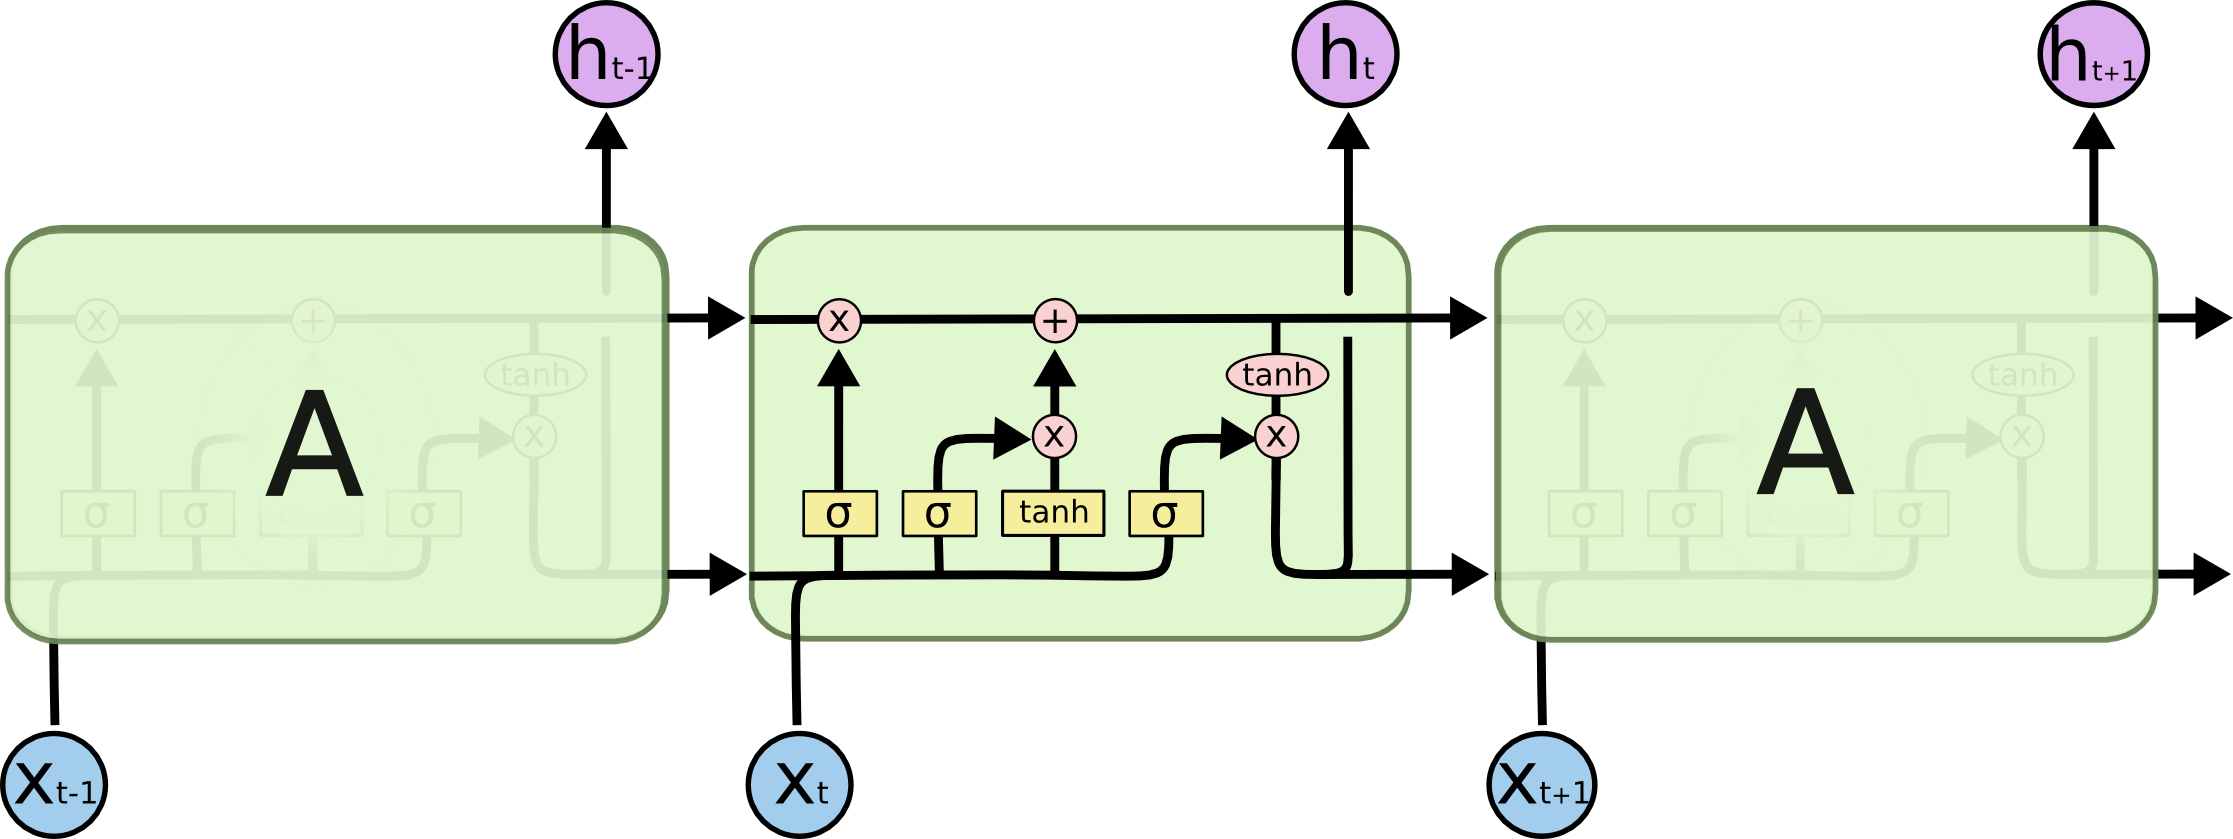
\includegraphics[width=4.5in]{/home/chad/projex/olcmen/paper/LSTM3-chain.png}
    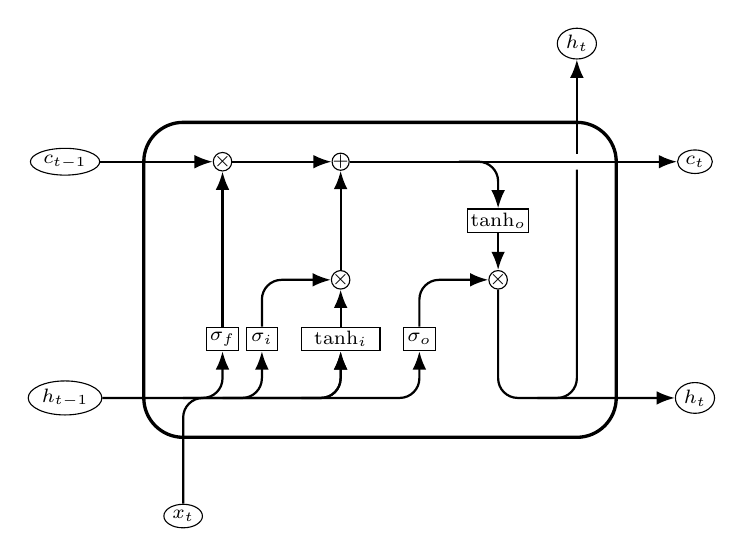
\begin{tikzpicture}[
    % GLOBAL CFG
    font=\sf \scriptsize,
    >=LaTeX,
    % Styles
    cell/.style={% For the main box
        rectangle, 
        rounded corners=5mm, 
        draw,
        very thick,
        },
    operator/.style={%For operators like +  and  x
        circle,
        draw,
        inner sep=-0.5pt,
        minimum height =.2cm,
        },
    function/.style={%For functions
        ellipse,
        draw,
        inner sep=1pt
        },
    ct/.style={% For external inputs and outputs
        circle,
        draw,
        line width = .75pt,
        minimum width=1cm,
        inner sep=1pt,
        },
    gt/.style={% For internal inputs
        rectangle,
        draw,
        minimum width=4mm,
        minimum height=3mm,
        inner sep=1pt
        },
    mylabel/.style={% something new that I have learned
        font=\scriptsize\sffamily
        },
    ArrowC1/.style={% Arrows with rounded corners
        rounded corners=.25cm,
        thick,
        },
    ArrowC2/.style={% Arrows with big rounded corners
        rounded corners=.25cm,
        thick,
        },
    ]

%Start drawing the thing...    
    % Draw the cell: 
    \node [cell, minimum height =4cm, minimum width=6cm] at (0,0){} ;

    % Draw inputs named ibox#
    \node [gt] (ibox1) at (-2,-0.75) {$\sigma_f$};
    \node [gt] (ibox2) at (-1.5,-0.75) {$\sigma_i$};
    \node [gt, minimum width=1cm] (ibox3) at (-0.5,-0.75) {$\tanh_i$};
    \node [gt] (ibox4) at (0.5,-0.75) {$\sigma_o$};

   % Draw opérators   named mux# , add# and func#
    \node [operator] (mux1) at (-2,1.5) {$\times$};
    \node [operator] (add1) at (-0.5,1.5) {+};
    \node [operator] (mux2) at (-0.5,0) {$\times$};
    \node [operator] (mux3) at (1.5,0) {$\times$};
    \node [gt] (func1) at (1.5,0.75) {$\tanh_o$};

%    % Draw External inputs? named as basis c,h,x
%    \node[ct, label={[mylabel]Cell}] (c) at (-4,1.5) {\empt{c}{t-1}};
%    \node[ct, label={[mylabel]Hidden}] (h) at (-4,-1.5) {\empt{h}{t-1}};
%    \node[ct, label={[mylabel]left:Input}] (x) at (-2.5,-3) {\empt{x}{t}};
%
%    % Draw External outputs? named as basis c2,h2,x2
%    \node[ct, label={[mylabel]Label1}] (c2) at (4,1.5) {\empt{c}{t}};
%    \node[ct, label={[mylabel]Label2}] (h2) at (4,-1.5) {\empt{h}{t}};
%    \node[ct, label={[mylabel]left:Label3}] (x2) at (2.5,3) {\empt{h}{t}};

    % Draw External inputs? named as basis c,h,x
    %\node[function] (c) at (-4,1.5) {\empt{c}{t-1}};
    \node[function] (c) at (-4,1.5)  {$c_{t-1}$};
    \node[function] (h) at (-4,-1.5) {$h_{t-1}$};
    \node[function] (x) at (-2.5,-3) {$x_{t}$};

    % Draw External outputs? named as basis c2,h2,x2
    \node[function] (c2) at (4,1.5)  {$c_{t}$};
    \node[function] (h2) at (4,-1.5) {$h_{t}$};
    \node[function] (x2) at (2.5,3)  {$h_{t}$};

% Start connecting all.
    %Intersections and displacements are used. 
    % Drawing arrows    
    %\draw [->,ArrowC1] (c) -- (mux1) -- (add1) -- (c2);
    \draw [->,ArrowC1] (c) -- (mux1);
    \draw [->,ArrowC1] (mux1) -- (add1);
    \draw [->,ArrowC1] (add1) -- (c2);

    % Inputs
    \draw [->,ArrowC2] (h) -| (ibox4);
    \draw [->,ArrowC1] (h -| ibox1)++(-0.5,0) -| (ibox1); 
    \draw [->,ArrowC1] (h -| ibox2)++(-0.5,0) -| (ibox2);
    \draw [->,ArrowC1] (h -| ibox3)++(-0.5,0) -| (ibox3);
    \draw [->,ArrowC1] (x) -- (x |- h)-| (ibox3);

    % Internal
    \draw [->, ArrowC2] (ibox1) -- (mux1);
    \draw [->, ArrowC2] (ibox2) |- (mux2);
    \draw [->, ArrowC2] (ibox3) -- (mux2);
    \draw [->, ArrowC2] (ibox4) |- (mux3);
    \draw [->, ArrowC2] (mux2) -- (add1);
    \draw [->, ArrowC1] (add1 -| func1)++(-0.5,0) -| (func1);
    \draw [->, ArrowC2] (func1) -- (mux3);

    %Outputs
    \draw [->, ArrowC2] (mux3) |- (h2);
    \draw (c2 -| x2) ++(0,-0.1) coordinate (i1);
    \draw [ArrowC2] (h2 -| x2)++(-0.5,0) -| (i1);
    \draw [->, ArrowC2] (i1)++(0,0.2) -- (x2);

\end{tikzpicture}

    \caption{Long-Short Term Memory Unit}
    \label{fig:lstm}
\end{figure}

\subsubsection{Convolutional LSTM}
Given the success of the LSTM in making predictions from streaming data, Shi et. al. extended the LSTM cell to include 2D convolutional layers to preprocess the input and the output from the prior step.  Current image recognition ANNs are based on convolutional neural networks (CNN) which segment the image into smaller regularly spaced overlapping rectangles and take their dot product with each filter from a set of trained filters. The dot products are arranged into a vector whose length is given by the number of filters.  The dot products are then arranged vertically onto a tensor with the same shape as the original image minus a buffer zone due to the size of the overlap.  An illustration with four filters is shown in \cref{fig:convlayers}.  

Note that the filters can be generalized to 3 dimensions for a multi-channel image. Two of the dimensions would be the size in pixels of the rectangles, and the third dimension would be the number of color channels.  The dot product will still produce a one dimensional vector with length same as the number of filters.

The filters are trained to minimize the loss function which compares the output to the real values.

\begin{figure}
    %\pgfdeclarelayer{bottom}
%\pgfdeclarelayer{top}
%\pgfsetlayers{bottom,main,top}
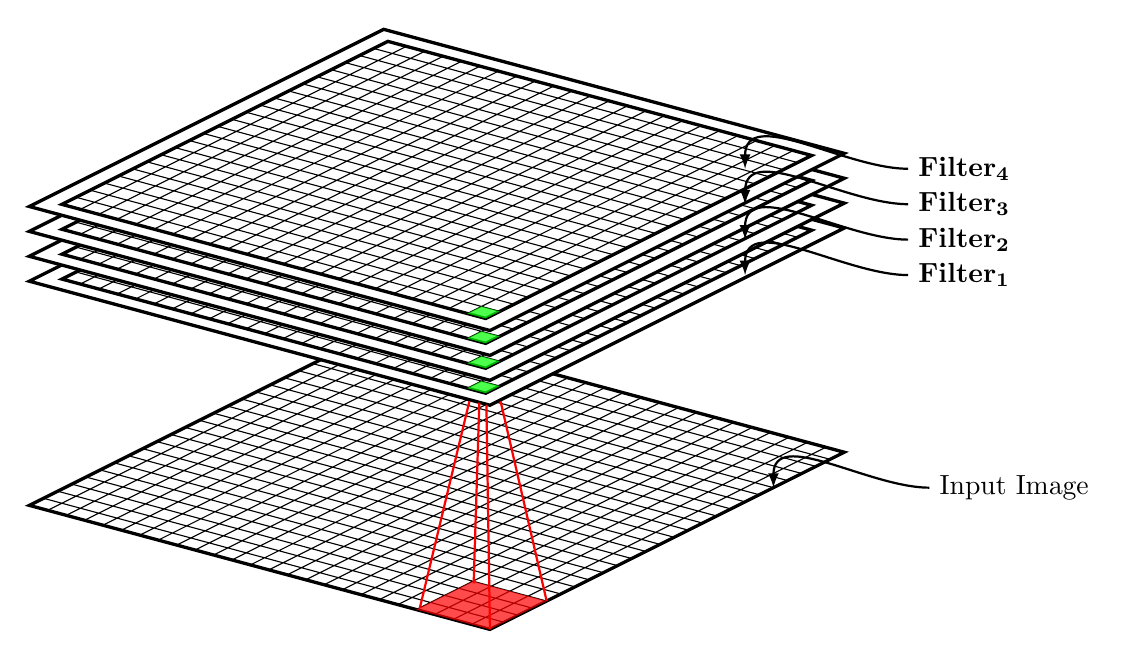
\begin{tikzpicture}[scale=.9,every node/.style={minimum size=1cm},on grid]
%    \begin{pgfonlayer}{bottom}
        \begin{scope}[
        	yshift=0,every node/.append style={
        	yslant=0.5,xslant=-1.3},yslant=0.5,xslant=-1.3]
            \fill[white,fill opacity=.9] (0,0) rectangle (5,5);
            \draw[black,very thick] (0,0) rectangle (5,5);
            \draw[step=2mm, black] (0,0) grid (5,5);
            \fill[red,fill opacity=.7] (0,0) rectangle (.8,.8);
            %\draw[red,very thick] (0,0) rectangle (1,1);
%            \node[red,rectangle,name=B,draw] at (0,0) {q};
        \end{scope}
%    \end{pgfonlayer}
    	
%    \begin{pgfonlayer}{top}
        \begin{scope}[
        	yshift=90,every node/.append style={
        	yslant=0.5,xslant=-1.3},yslant=0.5,xslant=-1.3]
        	\fill[white,fill opacity=1] (0,0) rectangle (5,5);
        	\draw[step=2mm, black] (.2,.2) grid (4.8,4.8);
        	\draw[black,very thick] (.2,.2) rectangle (4.8,4.8);
        	\draw[black,very thick] (0,0) rectangle (5,5);
            \fill[green,fill opacity=.7] (0.2,0.2) rectangle (.4,.4);
%            \node[red,name=A,rectangle,draw] (0.2,0.2) {Q};
%            \begin{pgfonlayer}{bottom}
%            \foreach \i in {north east,north west,south west,south east}
%                \draw (A.\i) -- (B.\i);
%            \end{pgfonlayer}
        \end{scope}
%    \end{pgfonlayer}
    	
    \begin{scope}[
    	yshift=100,every node/.append style={
    	yslant=0.5,xslant=-1.3},yslant=0.5,xslant=-1.3]
    	\fill[white,fill opacity=1] (0,0) rectangle (5,5);
    	\draw[step=2mm, black] (.2,.2) grid (4.8,4.8);
    	\draw[black,very thick] (.2,.2) rectangle (4.8,4.8);
    	\draw[black,very thick] (0,0) rectangle (5,5);
        \fill[green,fill opacity=.7] (0.2,0.2) rectangle (.4,.4);
    \end{scope}
    	
    \begin{scope}[
    	yshift=110,every node/.append style={
    	yslant=0.5,xslant=-1.3},yslant=0.5,xslant=-1.3]
    	\fill[white,fill opacity=1] (0,0) rectangle (5,5);
    	\draw[step=2mm, black] (.2,.2) grid (4.8,4.8);
    	\draw[black,very thick] (.2,.2) rectangle (4.8,4.8);
    	\draw[black,very thick] (0,0) rectangle (5,5);
        \fill[green,fill opacity=.7] (0.2,0.2) rectangle (.4,.4);
    \end{scope}
    	
    \begin{scope}[
    	yshift=120,every node/.append style={
    	yslant=0.5,xslant=-1.3},yslant=0.5,xslant=-1.3]
    	\fill[white,fill opacity=1] (0,0) rectangle (5,5);
    	\draw[step=2mm, black] (.2,.2) grid (4.8,4.8);
    	\draw[black,very thick] (.2,.2) rectangle (4.8,4.8);
    	\draw[black,very thick] (0,0) rectangle (5,5);
        \fill[green,fill opacity=.7] (0.2,0.2) rectangle (.4,.4);
    \end{scope}
    	
    %putting arrows and labels:
    \draw[-latex,thick] (6.2,2) node[right]{Input Image}
         to[out=180,in=90] (4,2);

    \draw[-latex,thick](5.9,5)node[right]{$\mathbf{Filter_1}$}
        to[out=180,in=90] (3.6,5);

    \draw[-latex,thick](5.9,5.5)node[right]{$\mathbf{Filter_2}$}
        to[out=180,in=90] (3.6,5.5);

    \draw[-latex,thick](5.9,6)node[right]{$\mathbf{Filter_3}$}
        to[out=180,in=90] (3.6,6);

    \draw[-latex,thick](5.9,6.5)node[right]{$\mathbf{Filter_4}$}
        to[out=180,in=90] (3.6,6.5);

    \draw[red,thick](-0.05,3.17) to (0,0);
    \draw[red,thick](0.15,3.22) to (0.8,0.4);
    \draw[red,thick](-0.29,3.22) to (-0.99,0.3);
    \draw[red,thick](-0.15,3.20) to (-0.23,0.65);

\end{tikzpicture}

    \caption{Convolutional Layer}
    \label{fig:convlayers}
\end{figure}

\subsection{Architecture Design}
Similar architectures were used for both the CFD data and the wind tunnel data.
\subsubsection{CFD Data}


\subsubsection{Wind Tunnel Data}

\section{Results}
The ANNs we built had the objective of predicting a single or multiple images from an input of multiple images.  In both the wind tunnel and CFD cases we built ANNs to predict the next image in a sequence of images.  In addition for the CFD case we built an ANN to predict a sequence of images between the central images of a sequence as a time step refinement predictor.

\subsection{Wind Tunnel Results}
\begin{itemize}
    \item   quantity of training data time history of some POD modes, determine minimal quantity of data
\end{itemize}

\subsubsection{Comparison to prior results with POD}
\begin{itemize}
    \item   POD requires large number of modes to reconstruct, high numbered modes have high frequency temporal 
\end{itemize}

\subsubsection{Next Frame Prediction}
\begin{figure}
    \includegraphics[width=5in]{/home/chad/projex/olcmen/convlstm/inputdecks/id_cfd_offset_01/images/frame_000.jpg}
    \caption{Predicting next frame from a stream.  Actual frames above, predicted below}
\end{figure}

\subsection{CFD Results}
\begin{itemize}
    \item   stuff
\end{itemize}

\subsubsection{Time step refinement study}
\begin{figure}
    \includegraphics[width=5in]{/home/chad/projex/olcmen/convlstm/inputdecks/id_cfd_10/images/frame_000.jpg}
    \caption{Predicting center frames from a sequence.  Actual frames above, predicted below}
\end{figure}

\begin{itemize}
    \item   stuff
\end{itemize}

\begin{table}
    \begin{center}
        \caption{Time Step Refinement CFD Architecture}
        \begin{tabular}{l|l|l|l}
            \hline
            Layer & filters & kernel size & strides\\
            \hline
            ConvLSTM2D      & 20 &   (2, 2)  & 1\\
            MaxPool3D       &    &   (1,2,2) &\\
            ConvLSTM2D      & 2  &   (2, 2)  & 1\\
            Conv2DTranspose & 10 &   (2, 2)  & 1\\
            Conv2DTranspose & 1  &   (3, 3)  & (2,2)\\
            Reshape & & (1,649,1065,1)&\\
        \end{tabular}
    \end{center}
\end{table}

\subsubsection{Next Frame prediction}

\begin{table}
    \begin{center}
        \caption{Next Frame CFD Architecture}
        \begin{tabular}{l|l|l|l}
            \hline
            Layer & filters & kernel size & strides\\
            \hline
            ConvLSTM2D      & 10 & (4, 4)    & 1\\
            ConvLSTM2D      & 10 & (4, 4)    & 1\\
            ConvLSTM2D      & 10 & (2, 2)    & 1\\

            Conv3D          & 20 & (3,4,4)   &  \\
            Conv3DTranspose & 10 & (1, 2, 2) & (1,1,1)\\
            Conv3DTranspose & 10 & (1, 4, 4) & (1,1,1)\\
            Conv3DTranspose & 10 & (1, 4, 4) & (1,1,1)\\
            Conv3DTranspose &  1 & (1, 4, 4) & (1,1,1)\\
        \end{tabular}

    \end{center}
\end{table}
\begin{itemize}
    \item   stuff
\end{itemize}
\section{Summary}

\begin{figure}
    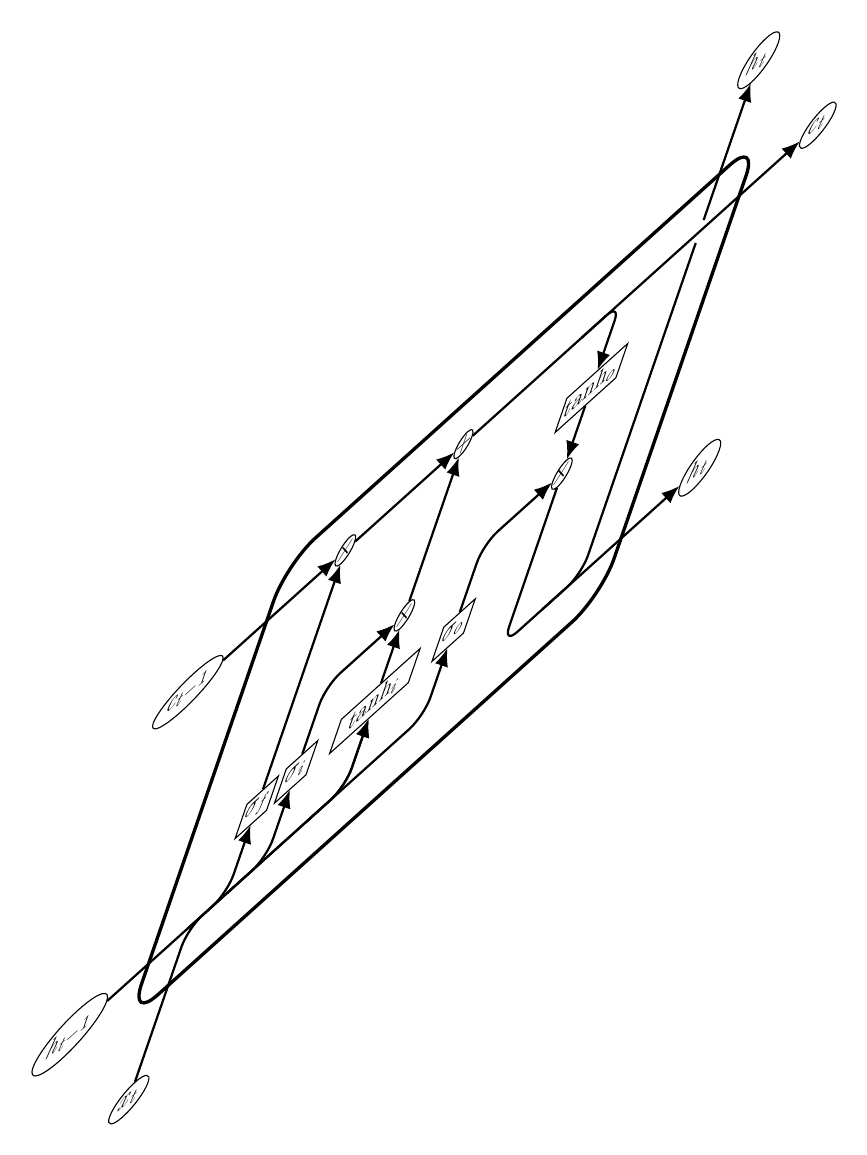
\begin{tikzpicture}[
    % GLOBAL CFG
    font=\sf \scriptsize,
    >=LaTeX,
    % Styles
    cell/.style={% For the main box
        rectangle, 
        rounded corners=5mm, 
        draw,
        very thick,
        },
    operator/.style={%For operators like +  and  x
        circle,
        draw,
        inner sep=-0.5pt,
        minimum height =.2cm,
        },
    function/.style={%For functions
        ellipse,
        draw,
        inner sep=1pt
        },
    ct/.style={% For external inputs and outputs
        circle,
        draw,
        line width = .75pt,
        minimum width=1cm,
        inner sep=1pt,
        },
    gt/.style={% For internal inputs
        rectangle,
        draw,
        minimum width=4mm,
        minimum height=3mm,
        inner sep=1pt
        },
    mylabel/.style={% something new that I have learned
        font=\scriptsize\sffamily
        },
    ArrowC1/.style={% Arrows with rounded corners
        rounded corners=.25cm,
        thick,
        },
    ArrowC2/.style={% Arrows with big rounded corners
        rounded corners=.25cm,
        thick,
        },
    ]

            %every node/.append style={yslant=-cot(45),xslant=-0.3},yslant=0.7,xslant=-0.3]
%Start drawing the thing...    
    % Draw the cell: 
    \begin{scope}
            [every node/.append style={yslant=0.9,xslant=0.5},yslant=0.9,xslant=0.5]
    {
        \node [cell, minimum height =4cm, minimum width=6cm] at (0,0){} ;
    
        % Draw inputs named ibox#
        \node [gt] (ibox1) at (-2,-0.75) {$\sigma_f$};
        \node [gt] (ibox2) at (-1.5,-0.75) {$\sigma_i$};
        \node [gt, minimum width=1cm] (ibox3) at (-0.5,-0.75) {$\tanh_i$};
        \node [gt] (ibox4) at (0.5,-0.75) {$\sigma_o$};
    
       % Draw opérators   named mux# , add# and func#
        \node [operator] (mux1) at (-2,1.5) {$\times$};
        \node [operator] (add1) at (-0.5,1.5) {+};
        \node [operator] (mux2) at (-0.5,0) {$\times$};
        \node [operator] (mux3) at (1.5,0) {$\times$};
        \node [gt] (func1) at (1.5,0.75) {$\tanh_o$};
    
    %    % Draw External inputs? named as basis c,h,x
    %    \node[ct, label={[mylabel]Cell}] (c) at (-4,1.5) {\empt{c}{t-1}};
    %    \node[ct, label={[mylabel]Hidden}] (h) at (-4,-1.5) {\empt{h}{t-1}};
    %    \node[ct, label={[mylabel]left:Input}] (x) at (-2.5,-3) {\empt{x}{t}};
    %
    %    % Draw External outputs? named as basis c2,h2,x2
    %    \node[ct, label={[mylabel]Label1}] (c2) at (4,1.5) {\empt{c}{t}};
    %    \node[ct, label={[mylabel]Label2}] (h2) at (4,-1.5) {\empt{h}{t}};
    %    \node[ct, label={[mylabel]left:Label3}] (x2) at (2.5,3) {\empt{h}{t}};
    
        % Draw External inputs? named as basis c,h,x
        %\node[function] (c) at (-4,1.5) {\empt{c}{t-1}};
        \node[function] (c) at (-4,1.5)  {$c_{t-1}$};
        \node[function] (h) at (-4,-1.5) {$h_{t-1}$};
        \node[function] (x) at (-2.5,-3) {$x_{t}$};
    
        % Draw External outputs? named as basis c2,h2,x2
        \node[function] (c2) at (4,1.5)  {$c_{t}$};
        \node[function] (h2) at (4,-1.5) {$h_{t}$};
        \node[function] (x2) at (2.5,3)  {$h_{t}$};
    
    % Start connecting all.
        %Intersections and displacements are used. 
        % Drawing arrows    
        %\draw [->,ArrowC1] (c) -- (mux1) -- (add1) -- (c2);
        \draw [->,ArrowC1] (c) -- (mux1);
        \draw [->,ArrowC1] (mux1) -- (add1);
        \draw [->,ArrowC1] (add1) -- (c2);
    
        % Inputs
        \draw [->,ArrowC2] (h) -| (ibox4);
        \draw [->,ArrowC1] (h -| ibox1)++(-0.5,0) -| (ibox1); 
        \draw [->,ArrowC1] (h -| ibox2)++(-0.5,0) -| (ibox2);
        \draw [->,ArrowC1] (h -| ibox3)++(-0.5,0) -| (ibox3);
        \draw [->,ArrowC1] (x) -- (x |- h)-| (ibox3);
    
        % Internal
        \draw [->, ArrowC2] (ibox1) -- (mux1);
        \draw [->, ArrowC2] (ibox2) |- (mux2);
        \draw [->, ArrowC2] (ibox3) -- (mux2);
        \draw [->, ArrowC2] (ibox4) |- (mux3);
        \draw [->, ArrowC2] (mux2) -- (add1);
        \draw [->, ArrowC1] (add1 -| func1)++(-0.5,0) -| (func1);
        \draw [->, ArrowC2] (func1) -- (mux3);
    
        %Outputs
        \draw [->, ArrowC2] (mux3) |- (h2);
        \draw (c2 -| x2) ++(0,-0.1) coordinate (i1);
        \draw [ArrowC2] (h2 -| x2)++(-0.5,0) -| (i1);
        \draw [->, ArrowC2] (i1)++(0,0.2) -- (x2);}
    \end{scope}


\end{tikzpicture}

    \caption{Architecture}
    \label{fig:anncfdarch}
\end{figure}

\begin{figure}
    \pgfdeclarelayer{bottom}
%\pgfdeclarelayer{top}
\pgfsetlayers{bottom,main}
%\pgfsetlayers{bottom,main,top}   
\begin{tikzpicture}[scale=.9,every node/.style={minimum size=1cm},on grid]       
\begin{pgfonlayer}{bottom}
    \begin{scope}[  % Lower layer
        yshift=0,every node/.append style={
            yslant=0.5,xslant=-1,rotate=-10},yslant=0.5,xslant=-1,rotate=-10
          ]
        \fill[white,fill opacity=0.9] (0,0) rectangle (5,5);
        \draw[step=10mm, gray!70] (2,2) grid (5,5);
        \draw[step=3.33mm, green] (2,2) grid (3,3);
        \draw[gray,very thick] (2,2) rectangle (5,5);
        \draw[black,dashed] (0,0) rectangle (5,5);
        \node[name=B,draw,scale=0.9,green,very thick,text width=0.95,text height=0.95,inner sep=0pt,] at (2.525,2.525) {};
    \end{scope}
\end{pgfonlayer}

    \begin{scope}[  % Upper layer
        yshift=105,every node/.append style={
        yslant=0.5,xslant=-1,rotate=-10},yslant=0.5,xslant=-1,rotate=-10
                     ]
        \fill[white,fill opacity=.6] (0,0) rectangle (5,5);
        \draw[step=10mm, green] (1,1) grid (4,4);
        \node[scale=.9,draw,green,very thick,name=A,text width=3cm,text height=3cm,inner sep=0pt] at (2.5,2.5) {};
        \draw[black,dashed] (0,0) rectangle (5,5);
        \begin{pgfonlayer}{bottom}
        \foreach \i in {north east,north west,south west,south east}
          \draw (A.\i) -- (B.\i);
        \end{pgfonlayer}
    \end{scope}

\end{tikzpicture}

    \caption{Layers}
    \label{fig:test}
\end{figure}

\end{document}
